\documentclass{article}
\title{Thermal Noise of Resistors}
\author{Zachariah Sachs}
\usepackage{graphicx}
\usepackage{float}

\begin{document}
\maketitle
\section{Purpose}
In this laboratory
exercise, we took various measurements of electronic circuit
elements to investigate the statistical and stochastic nature of
thermal noise and to confirm the Nyquist Theorem.

\section{Theory and Methods}

Measurements involving electronic circuits are fundamentally
limited by the discrete particles which carry charge and their
random thermal motion. For an ensemble of a sufficiently large
number of charge particles, in this case electrons occupying
microstates bound to the nuclei of atoms in a metal conductor,
spontaneous fluctuations of their motion at equilibrium show
small changes in the macroscopic properties current and
potential over time giving rise to a noise spectrum. Taking the
Fourier transform of the noise spectrum returns a power
spectrum. That is, for any particular frequency, the magnitude
of its contribution to the infinite series of periodic functions
which approximate the noise spectrum, its Fourier series, gives
the power of the signal. The time-dependence of the signal is
shifted into the range from the domain. The power spectrum that
results gives a Gaussian distribution of the thermal
fluctuations in terms of their frequency. This distribution is
statistically useful. Also, since it is independent of time, it
does not focus particularly on the kinetic energy of the
fluctuating particles, which is in turn dependent on
tempurature, but on the underlying statistics of the random
fluctuations.

Beginning with Ohm's Law and taking into account that the
macroscopic observables, current and potential, are averages of
the random motion of charge carriers, we get a
relation\footnote{See procedure, equation (3).} between average
potential and the stochastic velocity of electrons. Since the
power spectrum is the mean-square voltage vs. frequency, we next
consider the power in a frequency bandwidth as the product of
the spectral density times the bandwidth. This spectral density
can be derived from the time-correlation function of the
trajectory of the stochastic variable, in this case the
potential, via the Weiner-Khintchine Theorem\footnote{See
procedure, equation (6).}. Using these two relations and
accounting for the physical properties of the materials being
analyzed, we arrive at the Nyquist Theorem: \begin{equation}
\langle V^2\rangle=4 k_B T R \Delta f, \end{equation} where
$k_B$ is Boltzmann's constant, $T$ is temperature, $R$ is
resistance, and $\Delta f$ is the frequency bandwidth.

To confirm the Nyquist Theorem, we performed various
measurements hoping to linearly fit the data with a factor of
Boltzmann's constant. Using a computer program connected to a
digital oscilloscope, we took measurements of the
root-mean-square (RMS) voltage as a function of
frequency\footnote{Though the raw data was technically a noise
spectrum in time, and was accompanied by a power spectrum in
frequency, the calculations needed to confirm the Nyquist
Theorem only require the RMS output, and so these spectra are
not included in this report.}. First confirmed that the RMS
voltage from a function generator was not frequency-dependent.
Then we took several measurements of the RMS voltage of a sine
function passed through an amplifier at different frequencies
toget the frequency-dependent gain characteristics of the
amplifier. Finally, we took several measurements of the RMS
voltage from various resistors passed through the amplifier.

\section{Data and Plots}

\subsection{Temperature}

The temperature was measured as $295 \pm 2$ K.

\subsection{Function Generator and Amplifier Noise}

We measured the noise from the function generator over seven
trials as 55.9 mV with a standard of deviation of less than 1\%
of the average value.

The amplifier output for various frequencies was measured over
three trials to a standard of deviation of less than 4\% of the
average value and is ploted below.

\begin{figure}[H] 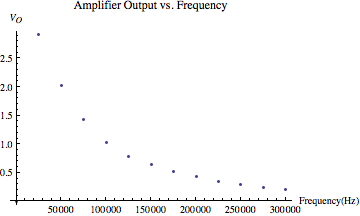
\includegraphics[width=0.8\textwidth]{vovf}
\centering \caption{The average amplifier gain characteristics
($V_O$ in volts) measured at frequency intervals of 25 kHz from
0 to 300 kHz.} \end{figure}

\subsection{Resistor Noise}

We measured the reference value of amplified resistor noise at
50 $\Omega$ over three trials as 17.9 mV with a standard of
deviation of less than 2\% of the average value.

The amplified noise of various resistors was measured over three
trials to a standard of deviation of less that 4\% of the
average value and is plotted below.

\begin{figure}[H] 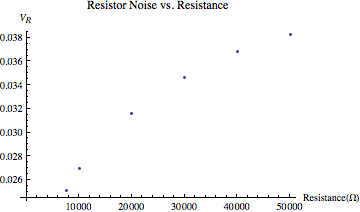
\includegraphics[width=0.8\textwidth]{vrvr}
\centering \caption{The average root-mean-square amplified
resistor noise measured for resistances of 7.5, 10, 20, 30, 40,
and 50 $k\Omega$ from a reference of 50 $\Omega$.} \end{figure}

\section{Analysis}

In order to get the frequency bandwidth $\Delta f$ as a function
of resistance $R$ exclusive of the gain from the amplifier, we
integrate numerically using the trapezoid rule: \begin{equation}
\Delta f(R)=\int_0^\infty \frac{(V_O(f)/V_i)^2}{1+(2\pi f R
C)^2} df. \end{equation} Here, $V_O$ is comes from the amplifier
gain characterisic shownin Figure 1, $V_i$ is the constant noise
from the function generator, $f$ is frequency, and $C$ is the
capacitance of the cable used to connect our circuit components.

The mean-square voltage as a function of resistance is given by
\begin{equation} \langle V^2\rangle=(\alpha V_R)^2-(\alpha
V_G)^2, \end{equation} where $V_R$ is the amplified resistor
noise from Figure 2, $V_G$is the reference resistance, and
$\alpha=0.01$ is a scale factorneeded to account for
amplification. This is plotted below.

\begin{figure}[H] 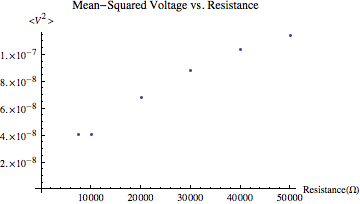
\includegraphics[width=0.8\textwidth]{MSVvR}
\centering \caption{The mean-square voltage of the resistors
adjusted for 40 dB amplification.} \end{figure}

According to equation (1) above, we expect a linear relation
between $\langle V^2\rangle/ \Delta f$ and frequency with a
slope of $4 k_B T$. The linear fit obtained is \begin{equation}
{\langle V^2\rangle}{\Delta
f}(R)=8.69\times10^{-17}+1.82\times10^{-20} R. \end{equation}
The data points and linear fit are plotted below. This fit gives
a value of $(1.82\times10^{-20}V s
\Omega^{-1})\div(4\cdot295K)=1.54\times10^{-23}J K^{-1}$ for the
Boltzmann constant, a deviation from the accepted value of
$1.38\times10^{-23}J K^{-1}$ of 11.7\%. \begin{figure}[H]
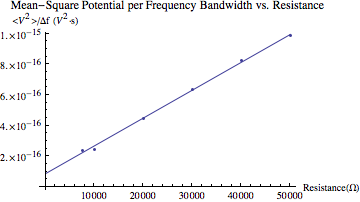
\includegraphics[width=0.8\textwidth]{Fit} \centering
\caption{The mean-square potential per frequency bandwidth
calculated using equations (2) and (3) at resistances of 7.5,
10, 20, 30, 40, and 50 $k\Omega$ from a reference of 50
$\Omega$.} \end{figure}

\section{Discussion}

The average value from the calculations above for the Boltzmann
constant is significantly above the accepted value. In terms of
data, this might be due to the number of frequencies at which we
measured the noise. We could have gotten a more precise gain
characteristic and value of $\Delta f$ if we had taken more
measurements. Indeed, integrating equation (2) using Simpson's
rule instead of the trapezoid rule gives an even higher
value\footnote{This calculation excluded.}. Also, during initial
measurements of resistor noise, we were getting an unwanted
periodic signal, perhaps from some electrical signal in the lab
which we were not able to discover. This extra ``noise'' would
tend to give a higher value of RMS voltage than expected.
Perhaps similar ambient noise remained when we took the gain
characteristic of the amplifier, and so we got high measurements
for $V_O$. This would give an inflated value of $\Delta f$, and
I think that based on the shape of the gain characteristic,
would give a larger slope than expected in the fit of
mean-square voltage per frequency bandwidth vs. resistance from
which we calculated Boltzmann's constant.

To minimize the uncertainty caused by resistor noise in any
measurement involving electronics, we would need to minimize the
resistance by various tricks. For example, we could operate the
electronics at low temperatures. For a fixed resistance, though,
this lab demonstrates that there is always a minimum abount of
noise fundamental to circuits.

This lab reveals another statistical-mechanical way of measuring
the Boltzmann constant, which is obviously fundamental to the
statistical-mechanics and thermodynamics, of chemistry. Noise in
circuit elements probably has heuristic parallels in
measurements of gases; for example, deviation from ideal-gas
behavior could be thought of as ``noise" due to random
fluctuation caused by interparticle forces.

\end{document}